
\section{Overview}
In this section, we present a comprehensive overview of our chosen methodologies, detailing their derivation and techniques. Our focus begins with the Vector Quantized Variational Autoencoder (VQVAE), an advanced model that represents an evolutionary step from the conventional Variational Autoencoder (VAE). We explore the foundational principles behind the VQVAE, including its development from the traditional VAE architecture, the core optimization challenges it addresses, and our approach to its implementation.

Further, we introduce a modified version of the VQVAE inspired by SSL and the Barlow Twins technique.


\section{The Vector Quantized Variational Auto-Encoder, VQVAE}

\subsection{Evolution from Variational Auto-Encoder, VAE}
The Vector Quantized Variational Autoencoder (VQ-VAE) evolves from the foundational principles of the Variational Autoencoder (VAE), sharing its dual-model architecture. 
At its core, a VAE consists of two models: the encoder, which compresses input data into latent representations, and the decoder, which reconstructs data from latent representations.
Giving rise to the bottleneck structure characterizing autoencoders.

As a fundemental principle of latent variable models, the Variational Autoencoder explicates the relationship between the observed data and latent variables through the marginal distribution. This relationship is central to understanding how a VAE encodes and decodes data, capturing the essence of the data's underlying structure.

Lets consider a dataset, denoted as $\mathbf{x}=\{x_1, x_2, \cdots, x_n \}$, which comprises observed data points. Corresponding to these data points, we have latent variables $\mathbf{z}=\{z_1, z_2, \cdots, z_n \}$, which represent hidden factors or features extracted by the VAE.
The model parameters denoted as $\theta$, govern the transformation from data to latent space and vice versa.

The relationship is explained by the marginal distribution, expressed as follows:

\begin{equation}
    p_\theta(x) = \int_zp_\theta(x, z) dz= \int_z p_\theta(z)p_\theta(x|z)dz    
\end{equation}

\subsubsection{Variational inference and optimization}
The optimization problem is to optimize $\theta$ to efficiently transform input data into a latent representation and reconstruct the input based on the latent representation.
Using the posteriors $p_\theta(\mathbf{z}|\mathbf{x})$ and $p_\theta(\mathbf{x}|\mathbf{z})$ both parameterized by $\theta$.
\subsubsection{Challenges in Maximum Likelihood Estimation}
Optimizing the model parameters \( \theta \) through Maximum Likelihood Estimation poses significant computational challenges. The optimization objective for \( \theta \) is to maximize the log likelihood of the observed data:

\begin{equation}
    \theta^* = \argmax_\theta \sum_{i=1}^n \log p(x_i | \theta)
\end{equation}

However, this requires evaluating an integral over the latent variables that is intractable:

\begin{equation}
    \theta^* = \argmax_\theta \sum_{i=1}^n \log\int_{z_i}p_\theta(x|z)p_\theta(z)
\end{equation}

\subsubsection{Variational Approximation}
To circumvent the intractability of the integral, we approximate the posterior \( p_\theta(z|x) \) with an encoder model \( q_\phi(z|x) \), parameterized by a neural network with variational parameters $\phi$, that maps the input data to the latent space.
The decoder neural network aims to reconstruct the input data $\mathbf{x}$, thereby approximating the conditional likelihood $p_\theta(\mathbf{x}|\mathbf{z})$.

\begin{equation}
    \mathbf{x}\rightarrow \underset{\sim q_\phi(\mathbf{z}|\mathbf{x})}{\text{EncoderNeuralNet}_\phi(\mathbf{x})} \rightarrow \mathbf{z} \rightarrow \underset{\sim p_\theta(\mathbf{x}|\mathbf{z})}{\text{DecoderNeuralNet}_\theta(\mathbf{z})} \rightarrow \hat{\mathbf{x}}
\end{equation}

\subsubsection{Evidence Lower Bound}
Due to the infeasibility of optimizing the likelihood directly it becomes necessary to adopt an alternative objective function. This function incorporates the variational aproximated posterior, $q_\phi(\mathbf{z}|\mathbf{x})$, and is commonly known as the Evidence Lower Bound (ELBO), denoted as $\mathcal{L}_{\theta, \phi}(x)$.

\begin{equation}
    \mathcal{L}_{\theta, \phi}(x) = \log p_\theta(x) - \mathcal{D}_{KL}(q_\phi(z|x) || p_\theta(z|x))
    \label{eq:ELBO}
\end{equation}

The first term in the ELBO, $\log p_\theta(x)$, represents the log likelihood of the data under the model parameters $\theta$. This term encourages the reconstructed data $\hat{\mathbf{x}}$, generated by the decoder network, to be as close as possible to the original input data $\mathbf{x}$.
The second term, 
\begin{equation}
\mathcal{D}_{KL}(q_\phi(z|x) || p_\theta(z|x))
\end{equation}
is the Kullback-Leibler (KL) divergence between the approximate posterior distribution $q_\phi(\mathbf{z}|\mathbf{x})$ and the true underlying distribution, $p_\theta(\mathbf{z}|\mathbf{x})$.

By maximizing the ELBO with respect to \( \theta \) and \( \phi \) we achieve the following:

\begin{enumerate}
    \item Enhancement of the marginal likelihood \( p_\theta(x) \), leading to improved reconstruction of the input data by the decoder.
    \item Reduction of the Kullback-Leibler (KL) divergence between the approximate posterior \( q_\phi(z|x) \) and the true posterior \( p_\theta(z|x) \), resulting in a more accurate encoder model for the latent variables.
\end{enumerate}

By maximizing the ELBO, we get a two for one, we refine the model's parameters to enhance data reconstruction accuracy and improve the encoder's inference of the latent representations, aligning them more closely with the true assumed underlying distribution.\cite{VAE}
\subsection{Transition to discrete latent variables}
VQ-VAE retains the encoder-decoder structure but introduces a discrete twist. It employs a vector quantization mechanism that translates the continuous latent variables of a traditional VAE into discrete ones, denoted as $\mathbf{z_q}$

The fundamentak shift from continous to discrete latent variables influences the dynamics of the model. In a VAE, the priors and posteriors are typically assumed gaussian. This assumption enables the application of the reparameterization trick\cite{1312.6114}, which is beneficial for effective training, primarily due to its contribution to
reducing gradient variance. However its important to note that this approach imposes a constraint that both the prior and posterior must conform to the underlying assumption of its shapes. This requirement, while beneficial for certain aspects of training, introduces a limitation in the models flexibility to represent a wider variety of data distributions.


\subsubsection{Vector quantization}
Vector quantization (VQ) is a key component of the VQ-VAE model, first proposed by van den Oord et al\cite{neuvqvae}. Within the architecture of the VQ-VAE, the encoder transforms input data into a series of continuous latent vectors. These vectors are then discretized through vector quantization,
which maps each continuous vector to the closest embedding vector in a predefined set known as the codebook.

The codebook, denoted by $\Zstroke$, is composed of $K$ discrete embedding vectors (or tokens), expressed as $\Zstroke = \{z_k\}_{k=1}^K$. Here $K$ represents the cardinality of the discrete latent space,
implying that the latent space comprises K distinct categories. Each embedding vector $z_k$ resides in a $d$-dimensional space. $z_k \in \R^d$

Quantization is implemented through a nearest neighbor search within $\Zstroke$. For any given continuous latent vector $z_{ij}$, the quantized vector $(z_q)_{ij}$ is determined by locating the token $z_k \in \Zstroke$ that minimizes the euclidian distance to $z_{ij}$.

$$(z_q)_{ij} = \argmin_{z_k \in \Zstroke}|| z_{ij} - z_k ||$$

\subsubsection{Effect on KL divergence}
As Van den Oord et al describes in their paper \cite{neuvqvae} each latent vector index maps deterministically to a single embedding vector in the codebook. As a result, the probability distribution of the latent indices given any input is a one-hot distribution. 
This means that for any given input, the posterior assigns a probability of one to a single latent index and zero to all others. 
\begin{equation}
    q(z = z_q | x) =
    \begin{cases}
    1 & \text{if } q = \argmin_{z_q \in \Zstroke} || z_{ij} - z_q || \\
    0 & \text{otherwise}
    \end{cases}
\end{equation}
(Stemmer formuleringen her??)

We can investigate the effects on the KL divergence by viewing the model as a VAE, as Van den Oord in his paper. Meaning that we bound $\log p_\theta(x)$ by the ELBO $\mathcal{L}_{\theta, \phi}$.
By now defining a simple uniform distribution over $z$ and using the one-hot deterministic $q(z=q|x)$ we can derive the KL-divergence as follows

\begin{equation}
    \begin{aligned}
        \mathcal{D}_{KL}(q_\phi(z|x) || p_\theta(z)) &= \sum_i \underbrace{q(z=q|x)}_{=1} \log \frac{\overbrace{q(z=q|x)}^{=1}}{\underbrace{p(z=q)}_{\frac{1}{K}}} \\
        &= \log K
    \end{aligned}
\end{equation}
(Skriv om .. Noen bruker p(z) andre p(z|x) for Kullback. Brukte p(z|x) i ELBO)

The constant KL divergence indicates a stable relationship between the aproximate posterior and the prior. The relationship is stable regardless of any assumption of shapes and forms for the posterior. This efficiently
addresses the "posterior collapse" or "KL vanishing"\cite{posteriorcollapse} issue commonly encountered in traditional VAEs. Posterior collapse occurs when the latent variables become less informative as the decoder learns to ignore the information provided by the 
encoder. In VQVAE, by allowing the posterior to take any shape without being bound by the constraints of a Gaussian distribution, the model maintains significance of the latent variables throughout training. 

\section{VQVAE implementation}
The implementation is based on the paper TimeVQVAE\cite{lee2023masked}. Here they argue for a 2 stage approach. The first stage consists of optimizing the Encoder, Codebook and Decoder to efficiently compress the input into tokens and then reconstruct the input.
This is achieved by minimizing the informational loss obtained by comparing the input $x$ with the reconstructed $\hat{x}$. The next stage consists of training a transformer to approximate the prior.

Stage 1 aligns with our objectives. They base their implementation on a improved approach to VQVAE, designed to extract better high frequency information. We base our implementation on the naive VQVAE as we are interested in the general case for VQVAEs on timeseries.

\subsection{Informational flow}
Prior to the encoder denoted by $E$, the input $\mathbf{x}$ (a timeseries) is passed through a Short Time Fourier Transform (STFT), producing $\mathbf{u}$. 

The \textbf{STFT} converts the time-domain signal into a time-frequency representation. This transformation allows the encoder to analyze the signal in both time and frequency domains simultaneously, providing a comprehensive view of the signal's spectral content as it varies over time. 
The encoder thus learns convolutional filters that capture and extract frequency patterns within the input data.
Reversly the Inverse Short Time Fourier Transform (\textbf{ISTFT}) converts the time-frequency representation back to a time-domain representation. 
Both STFT and ISTFT are computational methods grounded in a series of fourier transforms. A key parameter is $n_{\text{fft}}$, dictating the resolution of the frequencies in the transformed domain.

Next the encoder compresses $\mathbf{u}$ into a continuous latent variable $\mathbf{z}$ followed by a quantization to $\mathbf{z_q}$. Transforming the continous latent space to a discrete latent space. The input is at this state represented as tokens in our codebook.
The tokens or discrete latent variables is then passed through the decoder denoted as $D$, projecting the discrete latent space back into a time-frequency domain, $\hat{\mathbf{u}}$. Where it is then mapped back to a time-domain using ISTFT.
Giving the reconstructed input $\mathbf{\hat{x}}$. This is summerized in the figure \ref{fig:VQVAE}

\begin{center}
\begin{figure}[H]
    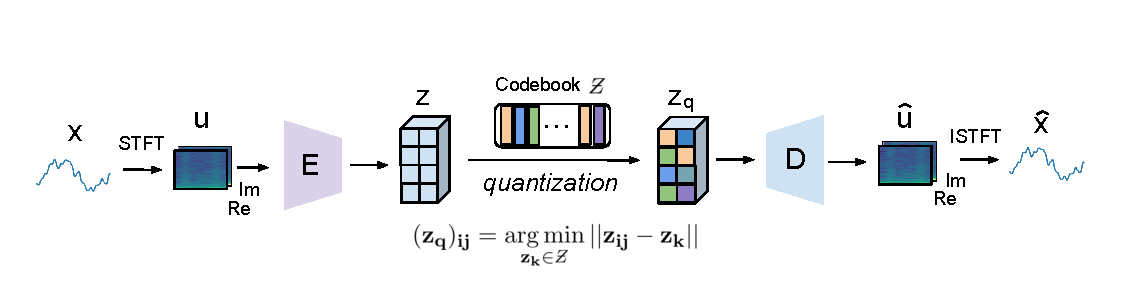
\includegraphics[scale=0.8]{figures/figure-pdf/VQVAE.pdf}
    \caption{ Illustration of the VQVAE. Illustration and implementation inspired by the TimeVQVAE paper\cite{lee2023masked} }
    \label{fig:VQVAE}
\end{figure}
\end{center}

\subsection{Learning}
Learning is achieved through updating the networks parameters through backpropagation. This process requires a formulation of a suitable loss function that reflects the learning objective of the model.

Based on the TimeVQVAE\cite{lee2023masked} paper and the ELBO formulation the total loss for the VQVAE is the sum of two parts. Reconstruction loss, $\mathcal{L}_{\text{recon}}$, and codebook loss, $\mathcal{L}_\text{codebook}$.
Contrary to the VAE, we dont have to include the minimization of the KL divergence.

\begin{equation}
    \mathcal{L}_{VQVAE} = \mathcal{L}_\text{recon} + \mathcal{L}_\text{codebook}
    \label{eq:VQVAEloss}
\end{equation}

\subsubsection{Reconstruction}
By minimizing the reconstruction loss, $\mathcal{L}_{\text{recon}}$, we align with maximization of $\log p_\theta(x)$ in the ELBO formulation \ref{eq:ELBO}.
We define the reconstruction loss to be:
\begin{equation}
    \mathcal{L}_{\text{recon}} = ||x-\hat{x}||_2^2 + ||u-\hat{u}||_2^2
\end{equation}

This gives us a metric or score on how well the reconstructed timeseries is compared to the input. As the metric acts on both time and time-frequency domain, we ensure that the 
model learns to reconstruct well for both of these domains.

To furhter clarify, the loss is calculated based on the Mean Squared Error (MSE), a standard metric in regression tasks. The MSE between the time domain input and reconstructed time domain input is defined as:
\begin{equation}
    MSE(x, \hat{x}) = \frac{1}{n} \sum_{i=1}^n (x_i - \hat{x}_i)^2
\end{equation}
Consequently, the reconstruction loss is expressed as the sum:
\begin{equation}
    \mathcal{L}_{\text{recon}} = MSE(x,\hat{x}) + MSE(u, \hat{u})
    \label{eq:recon}
\end{equation}

\subsubsection{Codebook-learning loss}
The codebook learning loss will ensure that the quantized latent representations, $\mathbf{z_q}$, effectively approximate the continues latent space $\mathbf{z}$, thereby maintaining a structured and meaning full latent representation. 

The codebook-learning loss is defined as
\begin{equation}
    \mathcal{L}_\text{codebook} = ||\text{sg}\left[ E(\text{STFT}(x))\right] - z_q||_2^2 + \beta|| E(\text{STFT}(x)) - \text{sg}\left[ z_q \right]||_2^2
\end{equation}

The first term in the codebook-learning loss,
\begin{equation}
    ||\text{sg}\left[ E(\text{STFT}(x))\right] - z_q||_2^2
\end{equation}
measures the difference between the stop-gradient, $\text{sg}\left[\cdot\right]$, aplied encoded representation and the quantized latent vector $z_q$. This term ensures that the chosen quantized vectors from the codebook are as close as possible to the output of the encoder. By applying the stop gradient operator, we prevent the gradients from backpropagating through the encoder during this part of the loss calculation.
Isolating the calculating to just act on the codebook network.

The second term,
\begin{equation}
    \beta|| E(\text{STFT}(x)) - \text{sg}\left[ z_q \right]||_2^2
\end{equation}
encourages the encoder's output to move closer to the quantized vectors. The parameter $\beta$ acts as a balanding factor, controlling the strength.  We typically set this parameter to be 1, ensuring that the encoder is updated at the same rate as the codebook.
(Kilde?). By applying the stop gradient on the quantized vector $z_q$, this term focuses on updating the encoder's parameters to produce outputs that are more aligned with the existing
codebook vectors.

Togheter, these two terms ensure that the codebook adapts to the encoded, $z$. Simultaneously, the encoder adapts to the quantized $z_q$. As a result the Encoder is tuned to produce representations that are effectively quantized by the codebook.
As done in the reconstruction loss the norms, $||\cdot||_2^2$, is replaced with MSE in our loss  calculation.
\section{Modifying the VQVAE for Enhanced Self Supervised Learning}
In this section we present our modification of the VQVAE, specifically tailored to leverage the strengths of Self Supervised Learning (SSL).
The primary goal of this modification is to build upon the existing VQVAE architecture, while adapting its encoder to produce more robust and informative latent representations.
To achieve this we propose the integration of the Barlow Twins method with the VQVAE encoder.


\subsection{Barlow Twins}
The Barlow Twins method, introduced by Zbontar et al in their 2021 article "Self-Supervised Learning via Redundancy Reduction"\cite{Barlow}, presents a alternative non-contrastive objective function for SSL. The core idea being an objective function that encourages the learning of feature representations
by reducing redundancy while retaining critical information from the input data. 

The rationale behind the objective function, $\mathcal{L}_{\text{BT}}$, is grounded in the properties of the identidy matrix. Viewing the identity matrix as a cross correlation matrix the zero valued off diagonal elements indicates no redundancy between different features. Since the diagonal elements are ones it suggest that each feature is similar, containing similar informational value.
Thereby, if a cross correleation matrix equals the identity matrix we have achieved no redundancy and full informative value between the features.

\subsubsection{Objective function of Barlow Twins}
The objective function, or similarity score, of the Barlow Twins method can be formulized as follows:

\begin{equation}
\mathcal{L}_{BT}(\mathbf{z_1}, \mathbf{z_2}) = \sum_i (1 - C_{ii})^2 + \lambda \sum_i \sum_{j \neq i} C_{ij}^2
\end{equation}

where $C$ is the cross correlation matrix computed between the outputs ($\mathbf{z_1}$ and $\mathbf{z_2}$) of two identical networks fed with distorted version of the same data (siamese style). $C_{ii}$ is the diagonal elements and $C_{ij}$ is the offdiagonal elements.
The parameter $\lambda$ controls the trade-off between invariance and redundancy reduction.

\subsubsection{Siamese architecture}
The barlow Twins method builds apon the siamese architecture, where each subnetwork consists of a encoder and a projector.

The procedure is as follows. First a batch normalization is applied to the distorted views ($Y^A$, $Y^B$) followed by a compression to latent variables by the Encoder, $E$. The projector, $P$, acts as a dimensionality expander with learnable parameters. It learns to expand the encodings into a space where the barlow twins loss can be efficiently applied.
The intuition behind expanding the dimensions is that more features in the cross-correlation matrix enable a more efficient and robust comparison while also allowing the model to capture a broader range of characteristics within the encodings.
Next the empirical cross correlation is compared with the Identity matrix as visualized in fig \ref{fig:Barlow}

\begin{figure}[H]
    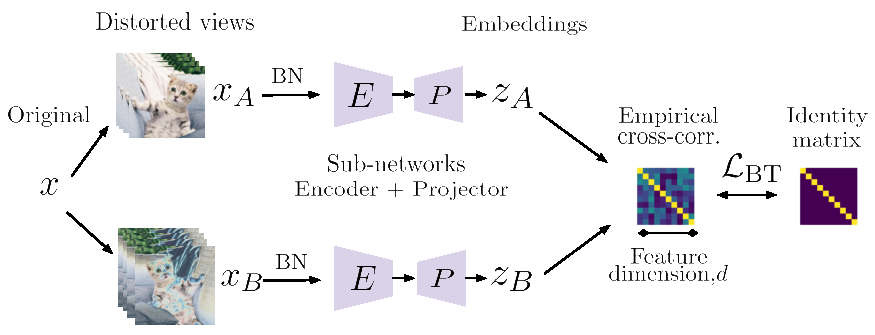
\includegraphics[scale=0.8]{figures/figure-pdf/BarlowT.pdf}
    \caption{Illustration of the Barlow Twins procedure, inspired by the original paper\cite{Barlow}.}
    \label{fig:Barlow}
\end{figure}

\subsection{Modifying the VQVAE encoder}
The proposed modification involves extending the VQVAEs encoder section into a two branch structure. Hence adopting a siamese architecture by augmenting 
the input $\mathbf{x}$ into two views, ($\mathbf{x_A}$, $\mathbf{x_B}$).

The same encoder in both branches then encodes both time-frequency views, ($\mathbf{u_A}$, $\mathbf{u_B}$). Producing two latent variables ($\mathbf{z_A}$, $\mathbf{z_B}$). We continue by calculating the barlow twins loss. First applying a batch normalization, $BN$, then using a projector denoted as $P$ to expand the dimensionality of the latent variables. As done by Zbontar et al in their paper\cite{Barlow}.
After the projection to a higher feature space, the cross correlation matrix, $C$, is calculated followed by the barlow twins loss function, $\mathcal{L}_{BT}$. This is summerized in fig \ref{fig:BTVQVAE}. 
As illustrated, the upper branch is the regular VQVAE and the lower branch is the extension allowing the encoder to process two views.

\begin{figure}[H]
    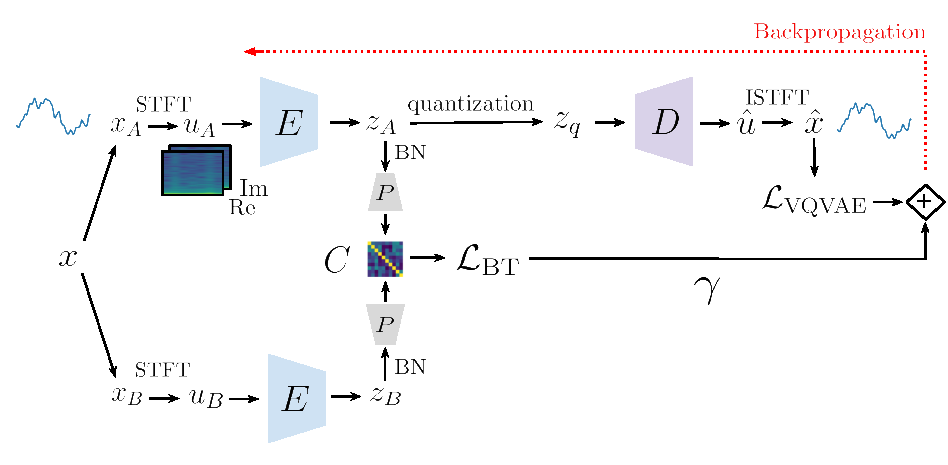
\includegraphics[scale=0.8]{figures/figure-pdf/BarlowTwinsVQVAE.pdf}
    \caption{Illustration of the Barlow Twins modification to VQVAE including the loss function calculation.}
    \label{fig:BTVQVAE}
\end{figure}

\subsubsection{Learning}
The modified VQVAE now has a additional SSL objective. As done by Bardes et al in their paper VICReg\cite{VICReg} we scale the barlow twins loss by the projected feature dimension, $d$, visualized in fig \ref{fig:Barlow}. Our Barlow Twins loss is extended as follows:

\begin{equation}
\mathcal{L}_{BT}(\mathbf{z_1}, \mathbf{z_2}) =\frac{1}{d} \left[ \sum_i (1 - C_{ii})^2 + \lambda \sum_i \sum_{j \neq i} C_{ij}^2\right]
\end{equation}

In the original barlow twins paper\cite{Barlow} they found that a low valued $\lambda$ equal to $0.005$ gave the optimal balance between invariance and redundancy reduction. They also found that the dimensionality of the projector had a substantial effect on the 
efficiency of the barlow twins loss calculation. A higher dimensionality gave better results. Based on this find, we expand the encoded dimension to $d=4096$ as done by Lee et al\cite{SSLs}. 

The total loss function, $\mathcal{L}_{\text{BT-VQVAE}}$, of our modified VQVAE becomes:

\begin{equation}
    \mathcal{L}_{\text{BT-VQVAE}} = \mathcal{L}_{\text{VQVAE}} + \gamma \cdot \mathcal{L}_\text{BT}
    \label{eq:BTVQVAEloss}
\end{equation}

The loss calculation is visualized in fig \ref{fig:BTVQVAE}. The parameter $\gamma$ determines the weight of the barlow twins loss in the calculation. The $\mathcal{L}_{VQVAE}$ is calculated as done in eq \ref{eq:VQVAEloss} using the upper branch reconstruction and codebook.


\subsection{Augmentation Techniques}
The augmentation techniques employed in this implementation, inspired by the paper by Wen et al\cite{augs} and the paper by Lee and Aune\cite{SSLs}, are categorized into time domain augmentations and time-frequency domain augmentations. 
A good augmentation should preserve overall schemantics of the timeseries during the transformation. 

\subsubsection*{Time Domain Augmentations}
These techniques manipulate the time series data directly in the time domain. A summerization of the implemented techniques are:
\begin{itemize}
    \item \textbf{Flipping}: Reversing the sequence of the time series, simulating time-reversed scenarios.
    \item \textbf{Jittering}: Adding Gaussian noise to the time series, introducing random variations akin to sensor noise or measurement errors.
    \item \textbf{Amplitude Resizing}: Adjusting the amplitude of the time series, simulating variations in signal strength.
    \item \textbf{Adding Slope}: Incorporating a linear trend, emulating gradual shifts or drifts in the data.
\end{itemize}

\subsubsection*{Time-Frequency Domain Augmentations}
These techniques operate on the time-frequency representation of the time series, offering a different perspective for augmentation:

\textbf{STFT Augmentation}: The most comprehensive technique in this implementation is the STFT (Short Time Fourier Transform) augmentation. It involves transforming the time series into the frequency domain using STFT, modifying the phase components using noise, and then reconstructing the time series. This process is particularly effective in introducing complex and subtle variations that are not easily achievable through direct time domain manipulations.

\begin{figure}[h]
    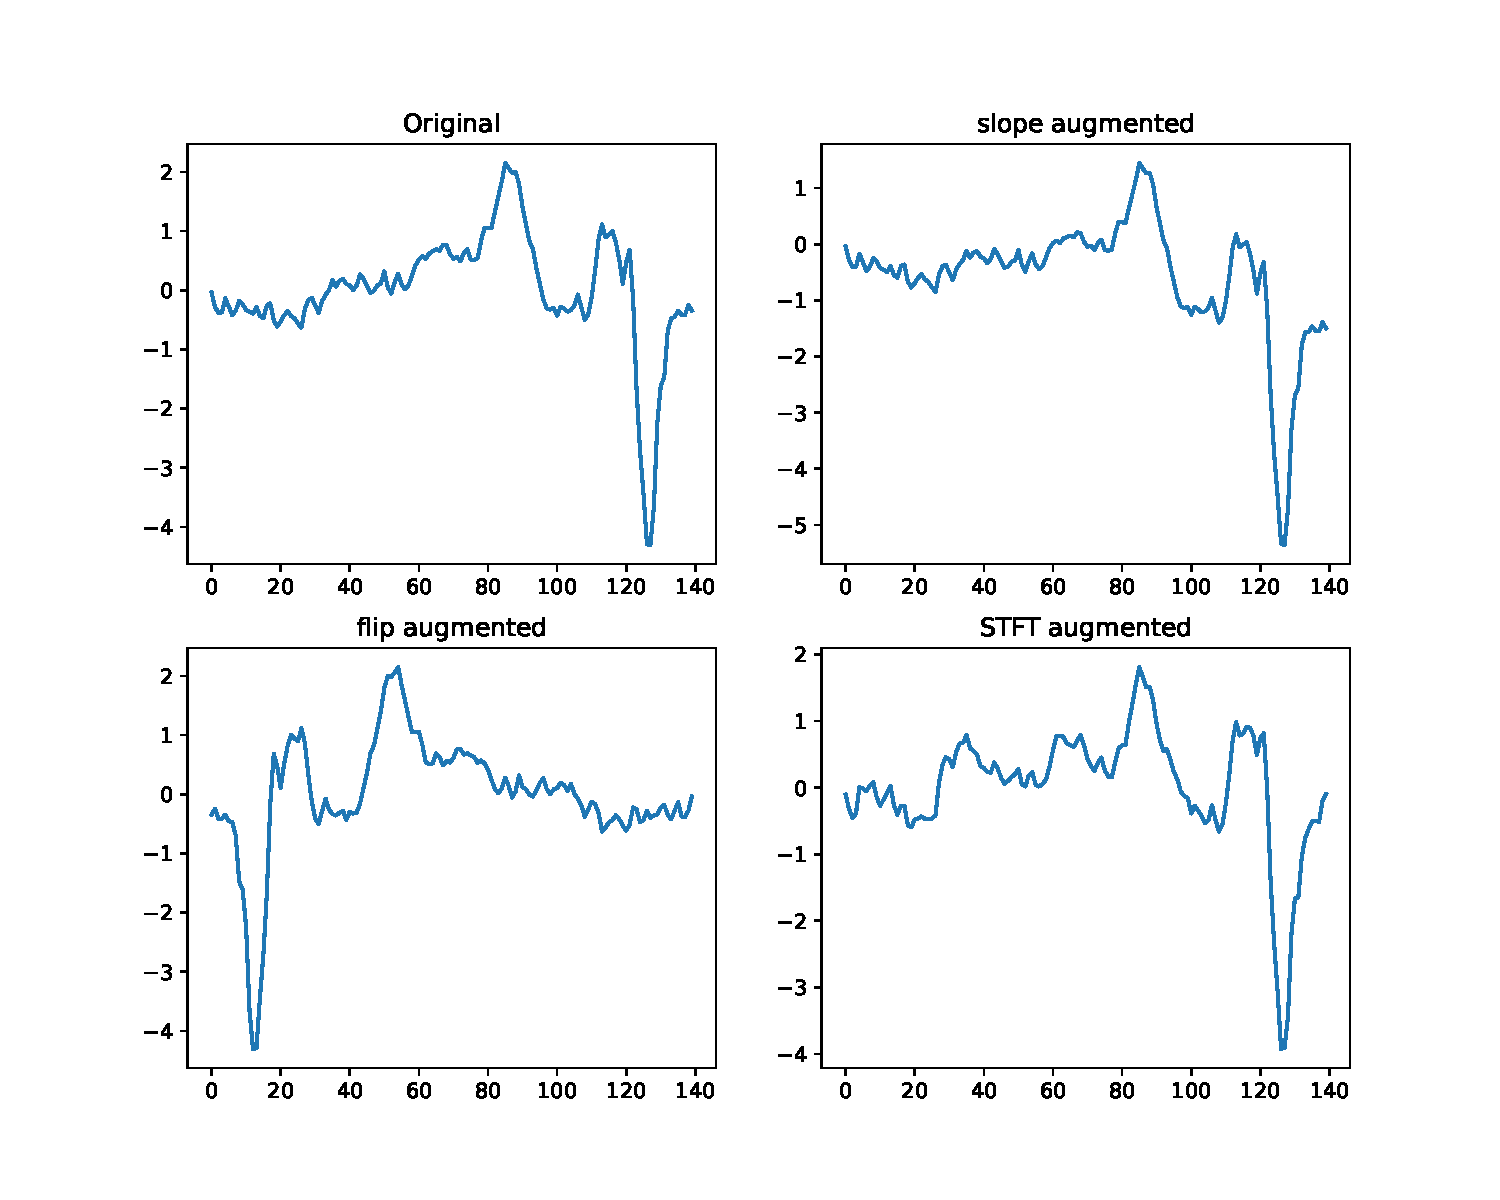
\includegraphics[scale=0.5]{figures/figure-pdf/Augmentations.pdf}
    \caption{Visualization of the flip, slope and STFT augmentation aplied on a timeseries. }
\end{figure}